% Iconic Wall Change Log — LaTeX typeset edition (Revision 5)
% Original Simons Center wall reference -> Mister Consistency fabrication artwork
\documentclass[10pt]{article}

\usepackage[margin=2.1cm,top=1.9cm,bottom=2.2cm]{geometry}
\usepackage[T1]{fontenc}
\usepackage[utf8]{inputenc}
\usepackage{newtxtext,newtxmath}
\usepackage{microtype}
\usepackage{graphicx}
\usepackage{booktabs}
\usepackage{tabularx}
\usepackage{longtable}
\usepackage{array}
\usepackage{ragged2e}
\usepackage{slashed}
\usepackage{fancyhdr}
\usepackage{enumitem}
\usepackage[hidelinks]{hyperref}
\usepackage{caption}

\captionsetup{font=small,labelfont=it,textfont=it}
\setlist[itemize]{leftmargin=1.35em,itemsep=2pt,topsep=3pt,parsep=0pt}

\newcolumntype{L}[1]{>{\RaggedRight\arraybackslash}p{#1}}

\pagestyle{fancy}
\fancyhf{}
\fancyfoot[L]{\small\itshape Iconic Wall Change Log \textbar\ prepared for Mister Consistency}
\fancyfoot[R]{\small\thepage\ of \pageref{LastPage}}
\renewcommand{\headrulewidth}{0pt}
\renewcommand{\footrulewidth}{0.4pt}
\usepackage{lastpage}

\setlength{\parindent}{0pt}
\setlength{\parskip}{3.4pt}

% compact section head: number+title over a hairline, minimal vertical cost
\newcommand{\head}[1]{\par\vspace{7pt}{\noindent\large\bfseries #1}\par
  \vspace{1pt}\noindent\rule{\linewidth}{0.4pt}\par\vspace{2pt}}

\begin{document}

% ============================================================ PAGE 1
\begin{center}
  {\LARGE\bfseries Iconic Wall Change Log}\\[3pt]
  {\large\itshape Original Simons Center wall reference $\rightarrow$ final
    Mister Consistency fabrication artwork}\\[2pt]
  {\footnotesize Revision 5 \,\textperiodcentered\, August 17, 2026 ---
    the five formulations we chose to restate, with our reasoning
    (\S3); full-page plates of the final and original walls\\[1pt]
  \footnotesize Rev.~4 (August 16, 2026) legend plaque caught up to the July 31
    artwork \,\textperiodcentered\, Rev.~3 (July 28, 2026) typeset edition
    \,\textperiodcentered\, Rev.~2 (July 9, 2026) Maxwell recast in
    differential forms; Bekenstein--Hawking added}
\end{center}
\vspace{-4pt}

\begin{figure}[h]
  \centering
  \begin{minipage}[c]{0.34\linewidth}
    \centering
    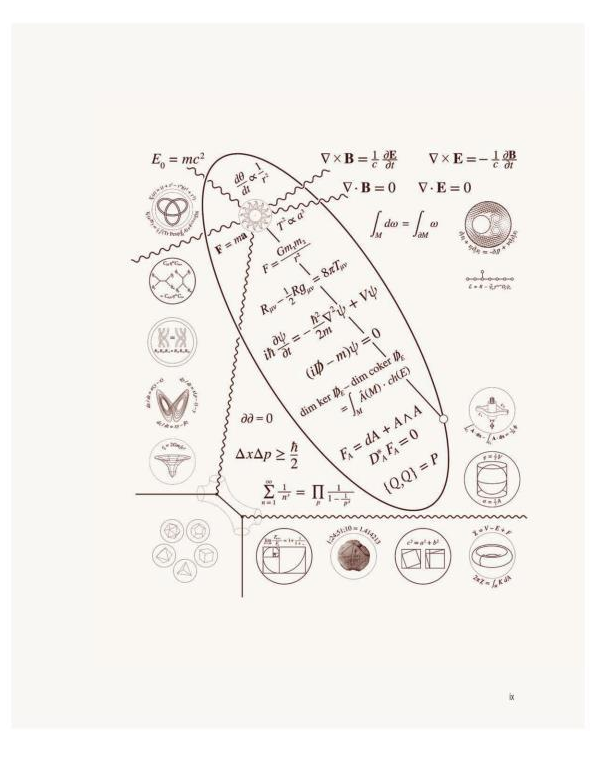
\includegraphics[height=5.35cm]{original-catalogue.png}\\[1pt]
    {\footnotesize Original reference diagram (catalogue)}
  \end{minipage}\hspace{0.045\linewidth}%
  \begin{minipage}[c]{0.42\linewidth}
    \centering
    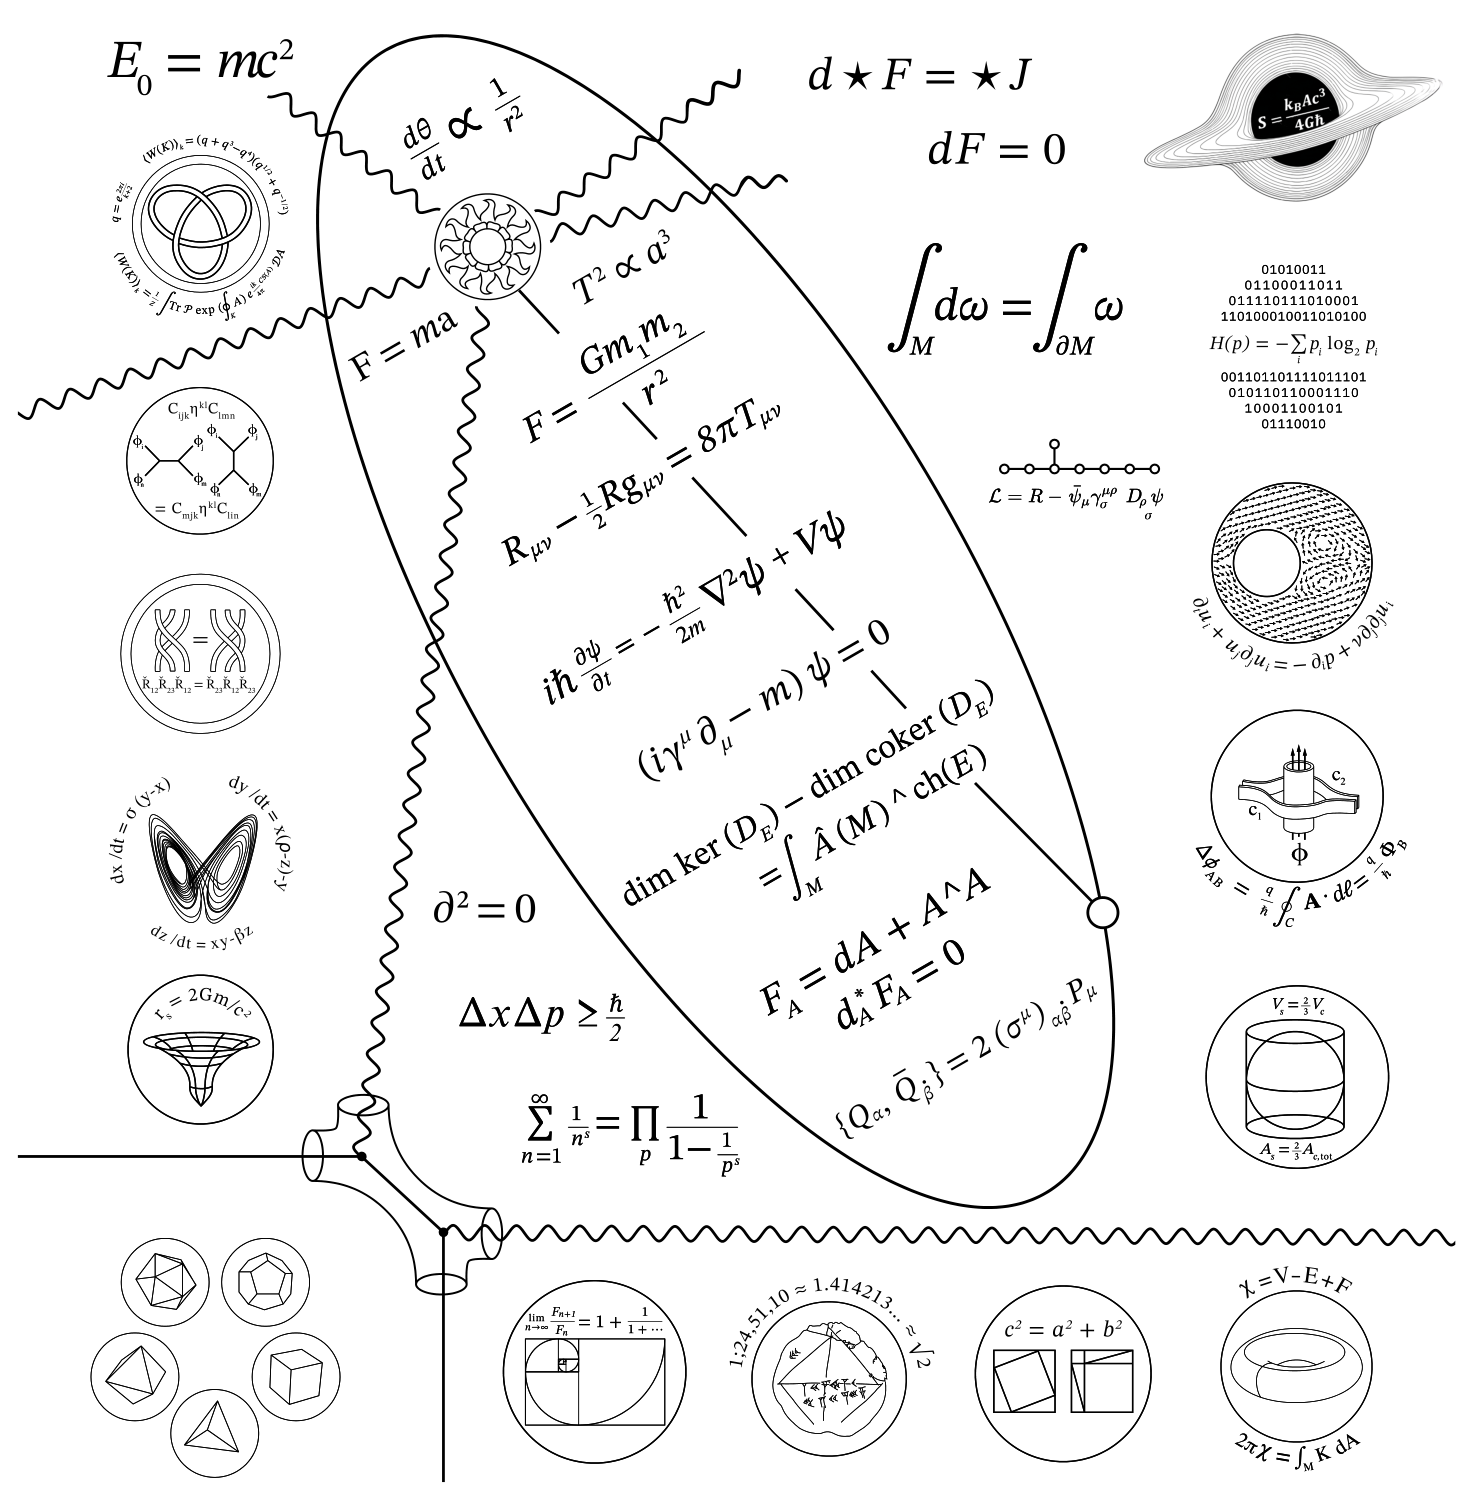
\includegraphics[height=5.35cm]{final-artwork.png}\\[1pt]
    {\footnotesize Final vector fabrication artwork (July 31, 2026)}
  \end{minipage}
  \vspace{-5pt}
  \caption{Original catalogue wall diagram beside the revised
    $42\times42$ vector fabrication artwork (July 31, 2026).}
\end{figure}
\vspace{-10pt}

\head{1\quad Executive summary}
\begin{itemize}
  \item The final Iconic Wall remains a faithful reconstruction of the
    original Simons Center wall: the central ellipse, peripheral
    medallions, background equations, and the wall's historical
    math--physics progression are all preserved.
  \item The dominant change is production-oriented: the stone-relief
    photographic reference was converted into monochrome,
    fabrication-ready vector line art for laser-etched or sandblasted
    steel panels ($42\times42$ and $32\times32$ inch, plus a
    $10\times10$ inch legend plaque).
  \item Two entries join the background --- Shannon's information theory
    (I) and the Bekenstein--Hawking entropy (J) --- expanding the
    background key from A--H to A--J, and Maxwell's equations are recast
    in differential forms. All three are told below.
  \item The July 31 artwork revision made J pictorial --- the formula
    now sits inscribed on the event horizon of a drawn black hole with
    accretion disc, top right --- and the legend plaque was revised to
    match (August 2026).
  \item The legend was rewritten for consistency and specificity:
    capitalization normalized, long entries shortened, credits tied to
    removed raster sources dropped, labels made precise. Several
    formulas were cleaned or clarified --- most notably Dirac,
    Yang--Mills, supersymmetry, Archimedes, boundary-of-boundary
    notation, and the mass--energy label.
  \item Revision 5 documents the five formulations we chose to
    restate, each with its reasoning (\S3). Headline: the Jones
    rewrite, previously logged as a redraw, is a deliberate change of
    notation ($V_K(t) \rightarrow \langle W(K)\rangle_k$). Full-page
    plates of both walls follow \S3; the detailed inventories now sit
    in the appendix.
\end{itemize}

\head{2\quad The three additions, in brief}

\textbf{B\quad Maxwell's equations, recast.}\enspace All of electricity,
all of magnetism, and light itself, in two short lines:
$\mathrm{d}F = 0$ and $\mathrm{d}{\star}F = {\star}J$. When Maxwell
first captured these laws in the 1860s they filled twenty equations;
vector calculus later compressed them to the famous four; the modern
language of differential forms --- the same $\mathrm{d}$ and $\star$
that appear elsewhere on this wall --- folds them into two. Physics got
deeper by getting shorter. The four vector-calculus equations of the
original wall are honored, not discarded: they are the same physics,
written in the wall's own geometric tongue.

\textbf{I\quad Shannon's information theory.}\enspace In 1948 a Bell
Labs engineer asked a question nobody thought was mathematics: how much
surprise does a message carry? Claude Shannon's answer,
$H(p) = -\sum_i p_i \log_2 p_i$, measures information in a brand-new
unit he named the \emph{bit} --- and drew a hard ceiling on how far any
message can be compressed and how fast any channel can carry it,
forever, regardless of technology. The raw binary carved around the
formula is the alphabet Shannon's theorem governs --- two symbols,
endlessly arranged, now carrying nearly all human communication.

\textbf{J\quad The Bekenstein--Hawking entropy.}\enspace One line, four
constants, four departments of physics:
$S = k_B A c^3\!/\,4G\hbar$ carries Newton's $G$ (gravity), Planck's
$\hbar$ (quantum), Einstein's $c$ (relativity), and Boltzmann's $k_B$
(thermodynamics). No other equation makes all four shake hands. It says
a black hole has entropy --- hidden information --- proportional to the
\emph{area} of its horizon, not the volume inside: everything a black
hole swallows is somehow recorded on its surface. Physicists call the
idea holography. The wall's newest stone, and its best candidate for
the physics of the next century.

% ============================================================ SECTION 3 (restated formulations)
\head{3\quad Restated and amended formulations}
The final wall does not reproduce every formula exactly as carved: in
five places we chose to restate a formulation. This section records
each decision: the original as it stands on the wall (quoted from the
official catalogue and checked against the carving; where the two
disagree, we say so), the form we adopted for the final artwork, and
the reasoning behind the choice. Immaterial differences of letterform
and spacing are inventoried in the appendix.

\subsection*{3.1\quad The Jones polynomial}
\textbf{Original} --- two arcs around the trefoil; the evaluation point
sits inside $V_K(\,\cdot\,)$:
\[ V_K(t) = (t + t^3 - t^4)\left(t^{\frac{1}{2}} + t^{-\frac{1}{2}}\right) \]
\[ V_K\!\left(e^{\frac{2\pi i}{k+2}}\right) = \frac{1}{Z}\int
   \left(\mathrm{Tr}\,\mathrm{Pexp}\oint_K A\right)
   e^{\frac{ik}{4\pi}\mathrm{CS}(A)}\,\mathcal{D}A \]
\textbf{Final} --- three formulas; the evaluation point becomes its own
statement:
\[ \langle W(K)\rangle_k = (q + q^3 - q^4)\left(q^{1/2} + q^{-1/2}\right)
   \qquad q = e^{\frac{2\pi i}{k+2}} \]
\[ \langle W(K)\rangle_k = \frac{1}{Z}\int
   \mathrm{Tr}\,\mathcal{P}\exp\!\left(\oint_K A\right)
   e^{\frac{ik}{4\pi}\mathrm{CS}(A)}\,\mathcal{D}A \]
\textbf{Why.}\enspace One statement, told in order. The bottom arc's
path integral computes a Wilson-loop expectation value, so the final
wall names the object honestly --- $\langle W(K)\rangle_k$, at level
$k$ --- instead of borrowing the polynomial's $V_K$. Pulling
$q = e^{2\pi i/(k+2)}$ out as its own formula states Witten's
dictionary explicitly (evaluate there, and the expectation value is the
Jones polynomial), letting the top arc give the trefoil's value in the
standard quantum variable $q$. Definition, dictionary, value --- three
arcs, one derivation. Script $\mathcal{P}$ marks path-ordering as an
operator rather than a field, and the parentheses now enclose exactly
what is exponentiated.

\subsection*{3.2\quad The boundary of a boundary is zero}
\[ \partial\partial = 0 \quad\longrightarrow\quad \partial^2 = 0 \]
\textbf{Why.}\enspace The squared form is the working statement of the
theorem: one operator, composed with itself, annihilating everything
--- which is how homology actually wields it, and how the rest of the
final wall already speaks (the exterior calculus of its Stokes and
Maxwell items, where $\mathrm{d}^2 = 0$ is the mirror identity).
$\partial\partial$ juxtaposes two symbols; $\partial^2$ asserts the
identity. Same truth, sharpened to its modern form.

\subsection*{3.3\quad The Dirac equation}
\[ (i\slashed{D} - m)\psi = 0 \quad\longrightarrow\quad
   (i\gamma^\mu \partial_\mu - m)\psi = 0 \]
\textbf{Why.}\enspace The slash is shorthand a reader must already own,
and the capital $\slashed{D}$ conventionally smuggles in a gauge field
--- leaving the carving suspended between the free equation and the
coupled one. The final wall writes the mechanism in full: gamma
matrices contracting the spacetime derivative, the Clifford square root
of the wave operator. That is Dirac's 1928 equation with nothing left
to convention; coupling then enters by the visible substitution
$\partial \rightarrow D$, not by silent capitalization.

\subsection*{3.4\quad The Yang--Mills equations}
\[ F = \mathrm{d}A + A \wedge A \qquad D_A^{*} F_A = 0
   \quad\longrightarrow\quad
   F_A = \mathrm{d}A + A \wedge A \qquad \mathrm{d}_A^{*} F_A = 0 \]
The stone carves the first $F$ bare; the catalogue's typeset panel
silently adds the subscript ($F_A$). The final wall follows the
catalogue.\par
\textbf{Why.}\enspace Two consistency repairs. The stone names the
curvature $F$ in line one and $F_A$ in line two; the final wall
subscripts both, so the object's dependence on the connection $A$ is
explicit and the pair closes on itself --- the $F_A$ annihilated in
line two is the $F_A$ defined in line one. And the operator family is
unified: line one builds curvature from the lowercase exterior
derivative $\mathrm{d}$; line two applies $\mathrm{d}_A^{*}$, the
adjoint of its covariant extension $\mathrm{d}_A$ --- staying in the
lowercase calculus where the original's uppercase $D_A^{*}$ switched
alphabets mid-pair. One connection, one calculus, one case.

\subsection*{3.5\quad Supersymmetry}
\[ \{Q, Q\} = P \quad\longrightarrow\quad
   \{Q_\alpha, \bar{Q}_{\dot{\beta}}\} =
   2(\sigma^\mu)_{\alpha\dot{\beta}} P_\mu \]
\textbf{Why.}\enspace The stone carves the catalogue's admitted
shorthand --- ``an equation for the operator $Q$'' --- with indices,
conjugation, and normalization all suppressed. The final wall carves
the theorem: in two-component form, supercharge and conjugate
supercharge close on the momentum through the sigma matrices. It is the
exact statement the slogan gestures at --- the square of a
supersymmetry is a translation --- now able to survive a reader who
checks the indices.

% ============================================================ PLATES
\newpage
\thispagestyle{fancy}
\begin{center}
  {\large\bfseries Plate 1\quad The final wall --- after}\\[2pt]
  {\footnotesize July 31, 2026 vector fabrication artwork, $42\times42$}\\[6pt]
  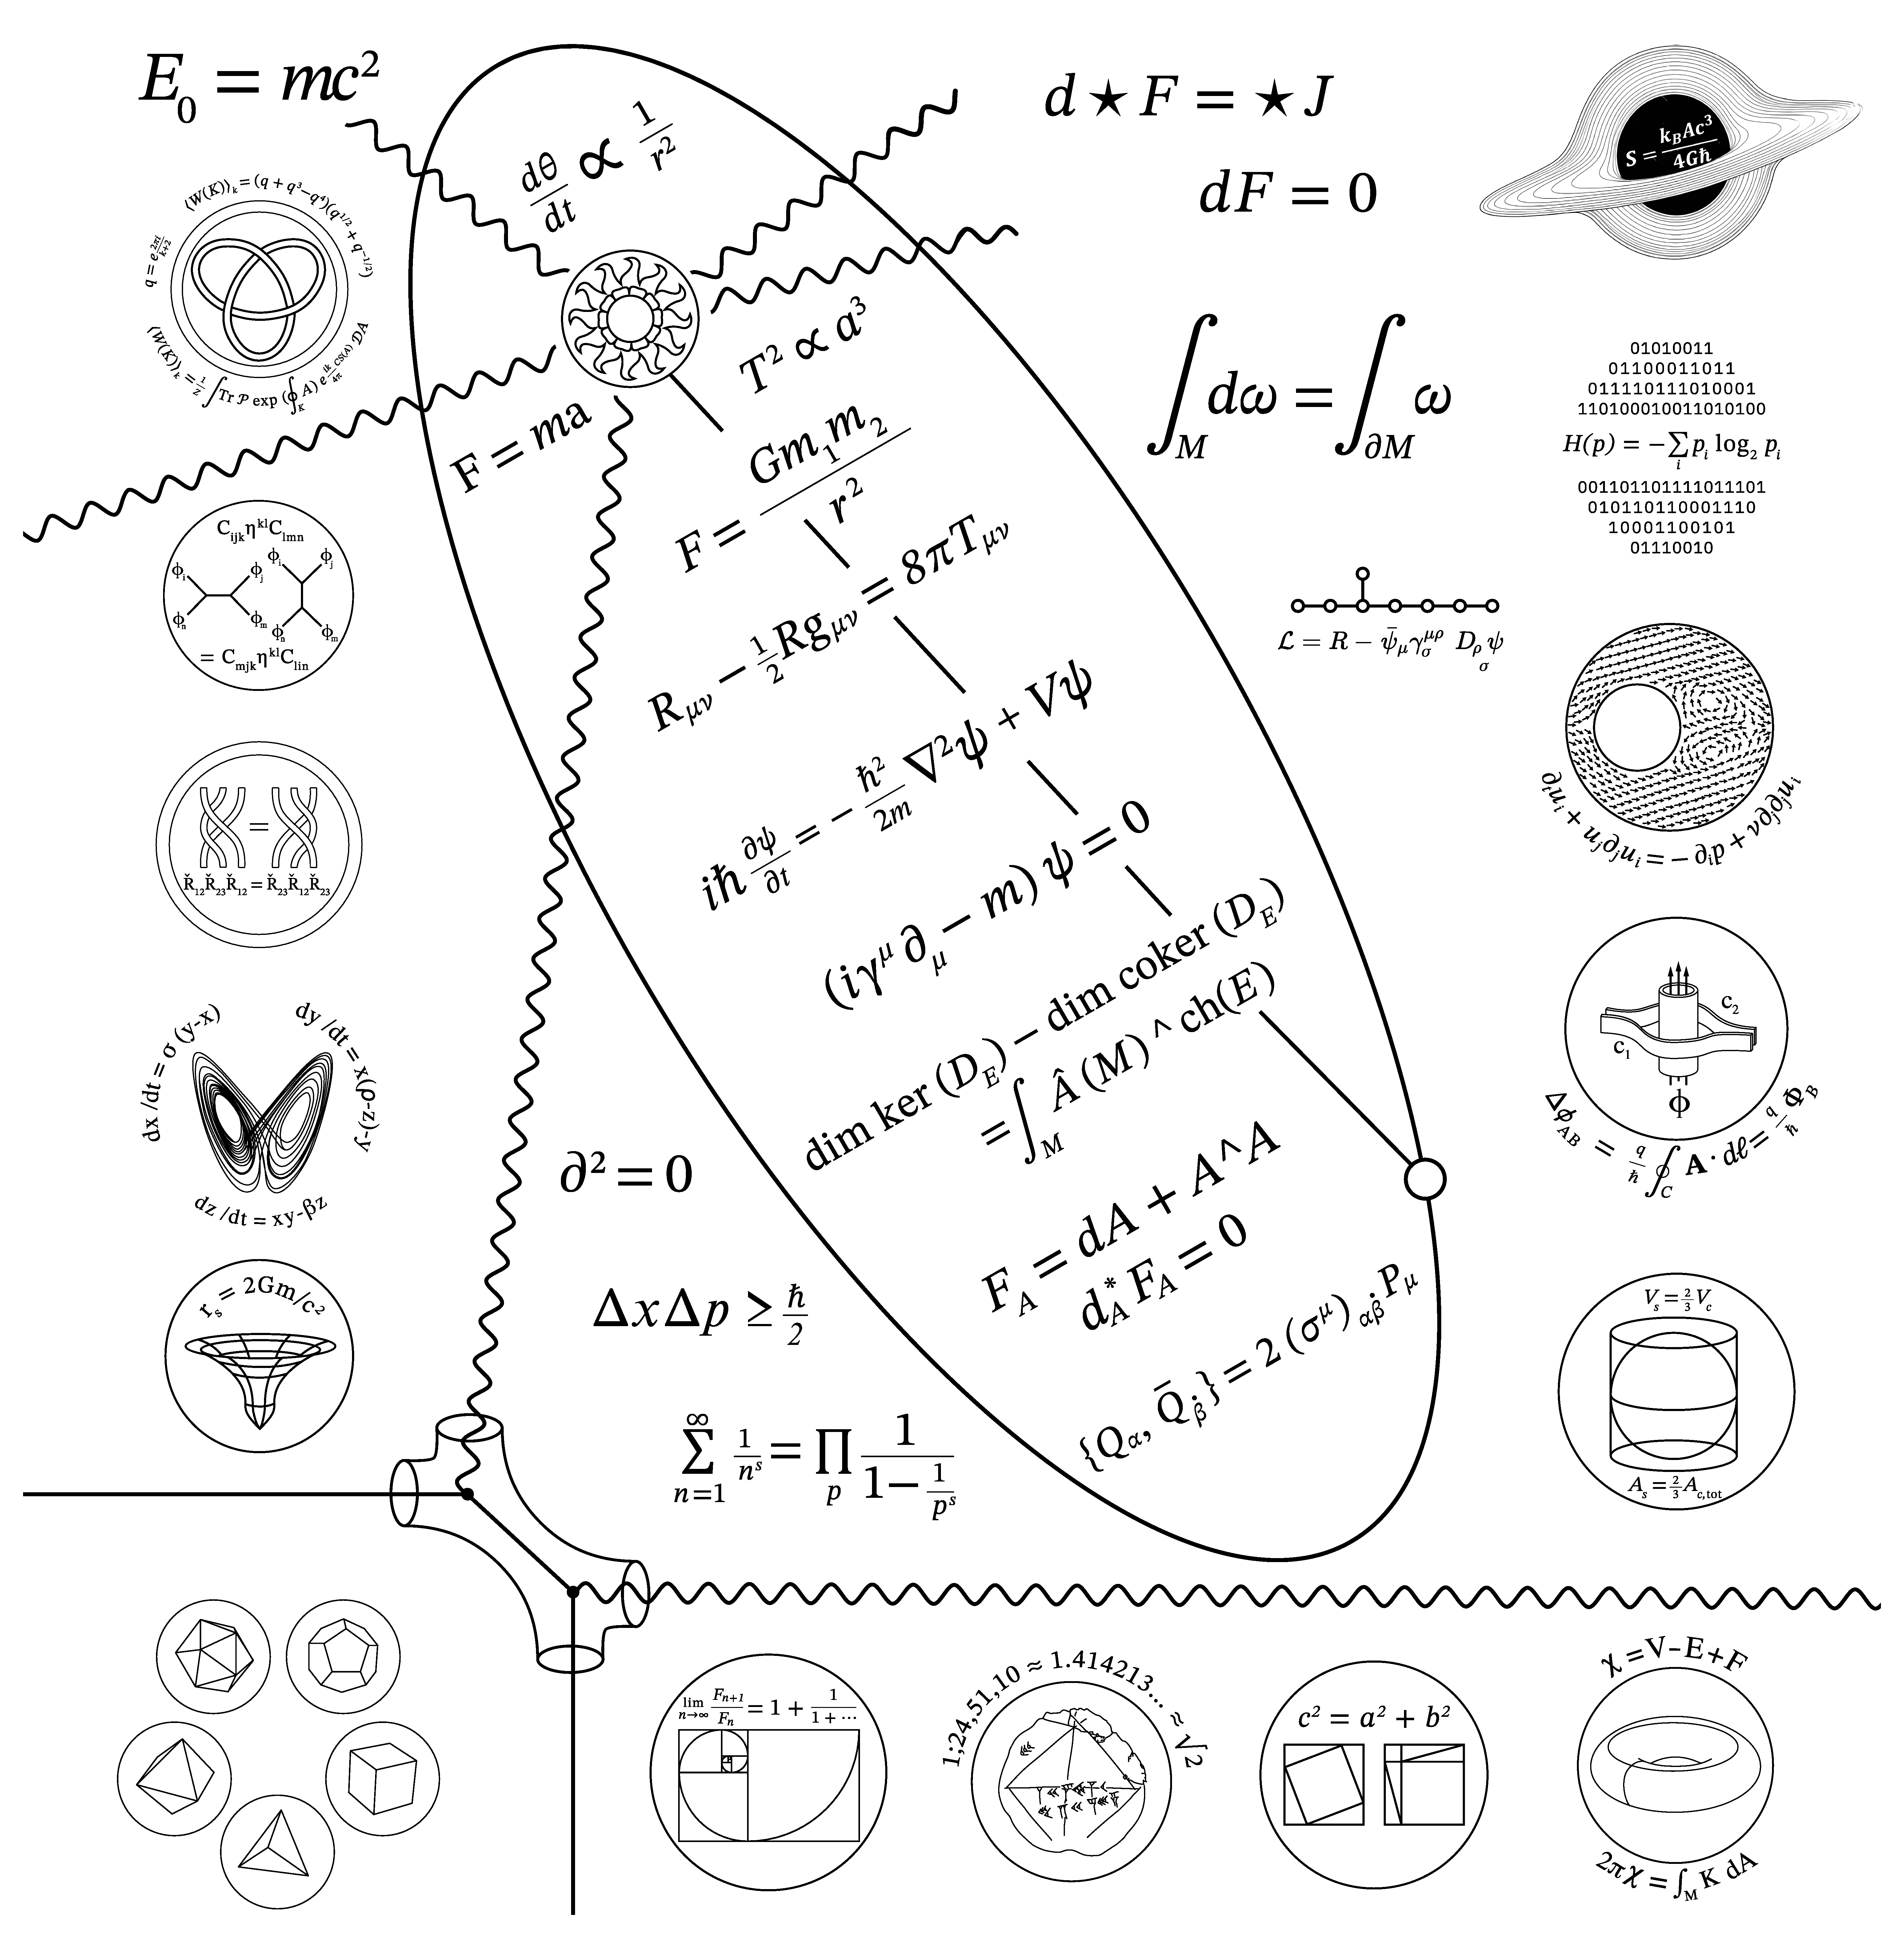
\includegraphics[width=\linewidth,height=0.88\textheight,keepaspectratio]{final-wall-73126.pdf}
\end{center}

\newpage
\thispagestyle{fancy}
\begin{center}
  {\large\bfseries Plate 2\quad The original Iconic Wall --- before}\\[2pt]
  {\footnotesize Simons Center for Geometry and Physics, Stony Brook ---
    carved limestone, dedicated May 8, 2015}\\[6pt]
  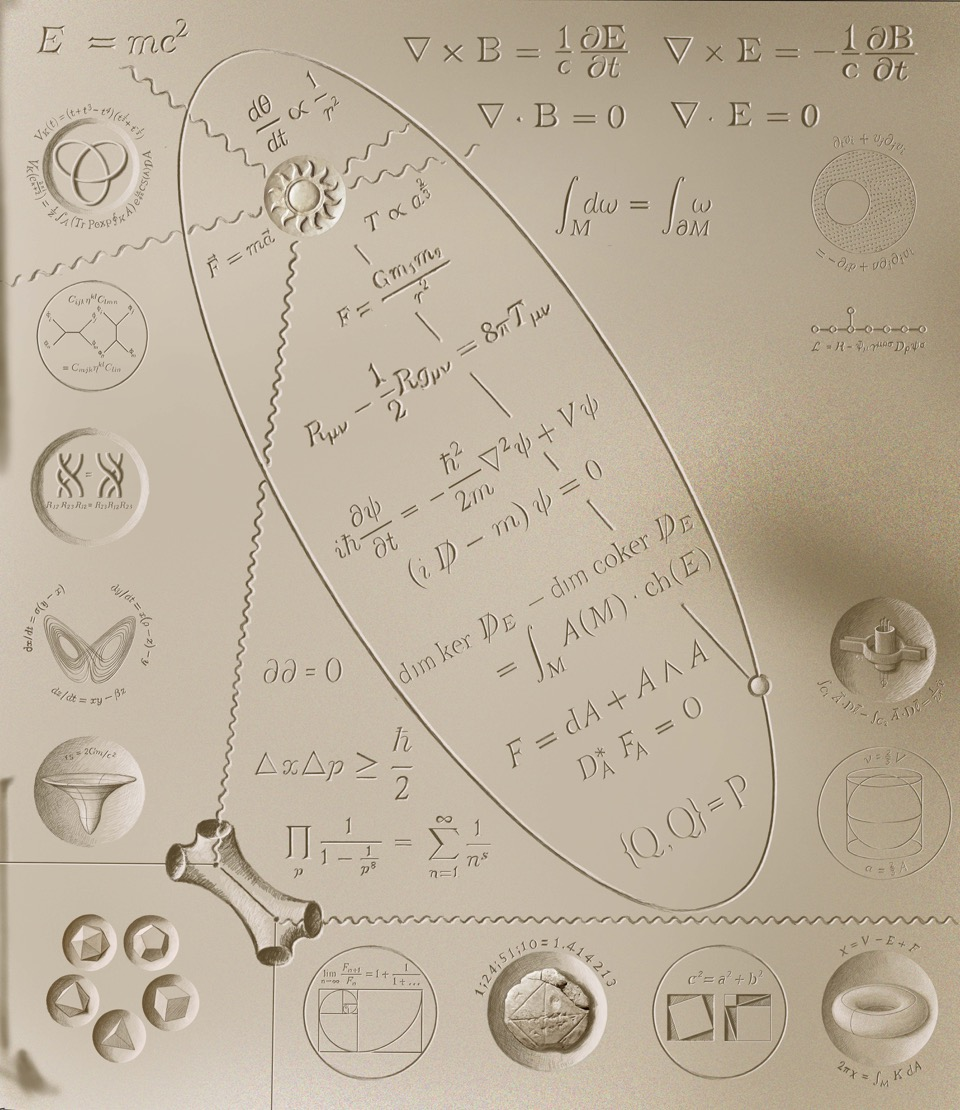
\includegraphics[width=\linewidth,height=0.88\textheight,keepaspectratio]{original-wall-full.jpg}
\end{center}

\newpage
% ============================================================ APPENDIX A
\head{Appendix A\quad Summary changes by category}
\renewcommand{\arraystretch}{1.25}
\begin{tabularx}{\linewidth}{@{}L{2.1cm} L{3.9cm} L{4.4cm} X@{}}
\toprule
\textbf{Area} & \textbf{Original} & \textbf{Final} & \textbf{Change made}\\
\midrule
Overall wall & Carved/sculpted wall documentation and catalogue diagram.
  & Rebuilt as clean, square, fabrication-ready vector line art.
  & Major production change: from photographic/relief reference to flat
    black vector art.\\
Overall format & Original installation is tall: $279\times240\times2$
    inches; the catalogue describes a $23\,\mathrm{ft}\times20\,\mathrm{ft}$ wall.
  & Square $42\times42$ and $32\times32$ inch panels, plus a
    $10\times10$ inch legend plaque.
  & Scale and aspect ratio changed for steel-panel fabrication.\\
Color / material & Stone relief, shadows, tonal texture, catalogue teal
    headings.
  & Pure black line art; no gradients, raster images, or shadows.
  & All tonal and material cues removed for engraving clarity.\\
All medallions & Mix of diagram line work, relief, and several
    photo-based medallions.
  & All medallions redrawn as consistent vector strokes.
  & Unifies style; improves reproducibility at reduced sizes.\\
Central ellipse & Large diagonal ellipse with sun, planet path, and
    equations 1--10.
  & Retained; line weights, spacing, and surrounding formulas cleaned
    for the square layout.
  & Core composition preserved.\\
Photon lines & Sculptural relief-like wavy lines crossing the wall.
  & Converted to a high-contrast vector stroke pattern.
  & Fabrication readability.\\
Background equations & Four vector-calculus Maxwell equations;
    background items A--H.
  & Maxwell recast as $\mathrm{d}F=0$, $\mathrm{d}{\star}F={\star}J$;
    Shannon (I) and Bekenstein--Hawking (J) blocks added.
  & Notation modernized; two new background entries.\\
Legend system & Key uses I--XIII, 1--10, and background A--H.
  & Key uses I--XIII, 1--10, and background A--J; plaque revised August
    2026 to mirror the July 31 layout, with J drawn as its black-hole
    silhouette.
  & The two additions required two new background key entries; locator
    updated to the current wall.\\
\bottomrule
\end{tabularx}

\vspace{10pt}
\head{Appendix B\quad Legend changes: original $\rightarrow$ final}
The final legend plaque is not a verbatim copy of the catalogue legend:
it is a rewritten key for a new fabrication object. The numbering
system remains; the wording is normalized and two background items are
added.

\renewcommand{\arraystretch}{1.22}
\begin{longtable}{@{}L{1.35cm} L{4.55cm} L{4.55cm} L{5.2cm}@{}}
\toprule
\textbf{Key} & \textbf{Original wording} & \textbf{Final wording} & \textbf{Change}\\
\midrule
\endhead
Heading & Key to Equations and Diagrams & Key to equations and diagrams
  (I--XIII) & Lowercase style normalized; numbering range made explicit.\\
I & The Jones Polynomial & The Jones polynomial & Capitalization normalized.\\
II & Associativity in Quantum Field Theory & Associativity in quantum
  field theory & Capitalization normalized.\\
III & The Yang-Baxter Equation & The Yang--Baxter equation &
  Capitalization normalized; dash treatment standardized.\\
IV & The Lorenz Attractor (Image: Scott Sutherland) & The Lorenz
  attractor & Capitalization normalized; image credit removed because
  the final is redrawn line art.\\
V & The Schwarzschild Black Hole & The Schwarzschild black hole &
  Capitalization normalized; spelling verified.\\
VI & The Five Platonic Solids & The five Platonic solids &
  Capitalization normalized.\\
VII & The Golden Ratio & The golden ratio & Capitalization normalized.\\
VIII & The Babylonian tablet YBC 7289 (Image: Bill Casselman) & The
  Babylonian tablet YBC 7289 & Raster-photo attribution removed; the
  final tablet is vector line art.\\
IX & The Pythagorean Theorem & The Pythagorean theorem &
  Capitalization normalized.\\
X & The Gauss-Bonnet Theorem & The Gauss--Bonnet theorem &
  Capitalization normalized; dash standardized.\\
XI & Archimedes' calculation of the volume and area of the sphere &
  Archimedes' sphere and cylinder & Long label shortened to the
  medallion's visual subject.\\
XII & The Aharonov-Bohm Effect & The Aharonov--Bohm effect &
  Capitalization normalized; dash standardized.\\
XIII & The Navier-Stokes Equations (Image: J.D. Kim, AMS, Stony Brook)
  & The Navier--Stokes equations & Capitalization normalized; image
  credit removed (redrawn as line art).\\
\addlinespace[2pt]
Ellipse heading & In the Ellipse & Within the ellipse (1--10) & Heading
  made natural; numbering range explicit.\\
Ellipse note & (Kepler's 1st law represented by star, ellipse, planet)
  & (Kepler's 1st law represented by star, ellipse, planet) & Kept;
  surrounding legend typography cleaned.\\
2 & Newton's Second Law of Motion & Newton's 2nd law of motion &
  Numeral style harmonized with Kepler's 1st/2nd/3rd laws.\\
\addlinespace[2pt]
Background heading & On the Background & On the background (A--J) &
  Capitalization normalized; expanded from A--H to A--J.\\
A & E=mc\textsuperscript{2} & Einstein's rest mass--energy equivalence
  & Formula-only label replaced with a descriptive title.\\
D & Supergravity & Minimal supergravity Lagrangian & Made specific to
  the displayed formula.\\
H & Feynman Diagrams & Feynman and string interaction
  ``pair-of-pants'' & Expanded to reflect the combined particle/string
  drawing.\\
I & \emph{No original entry} & Shannon's information theory & New
  background item added to the final artwork and legend.\\
J & \emph{No original entry} & Bekenstein--Hawking entropy & New
  background item added in the July 2026 revision; wording tightened
  and the locator glyph redrawn as the black hole with accretion disc
  (August 2026).\\
\bottomrule
\end{longtable}

\begin{figure}[h]
  \centering
  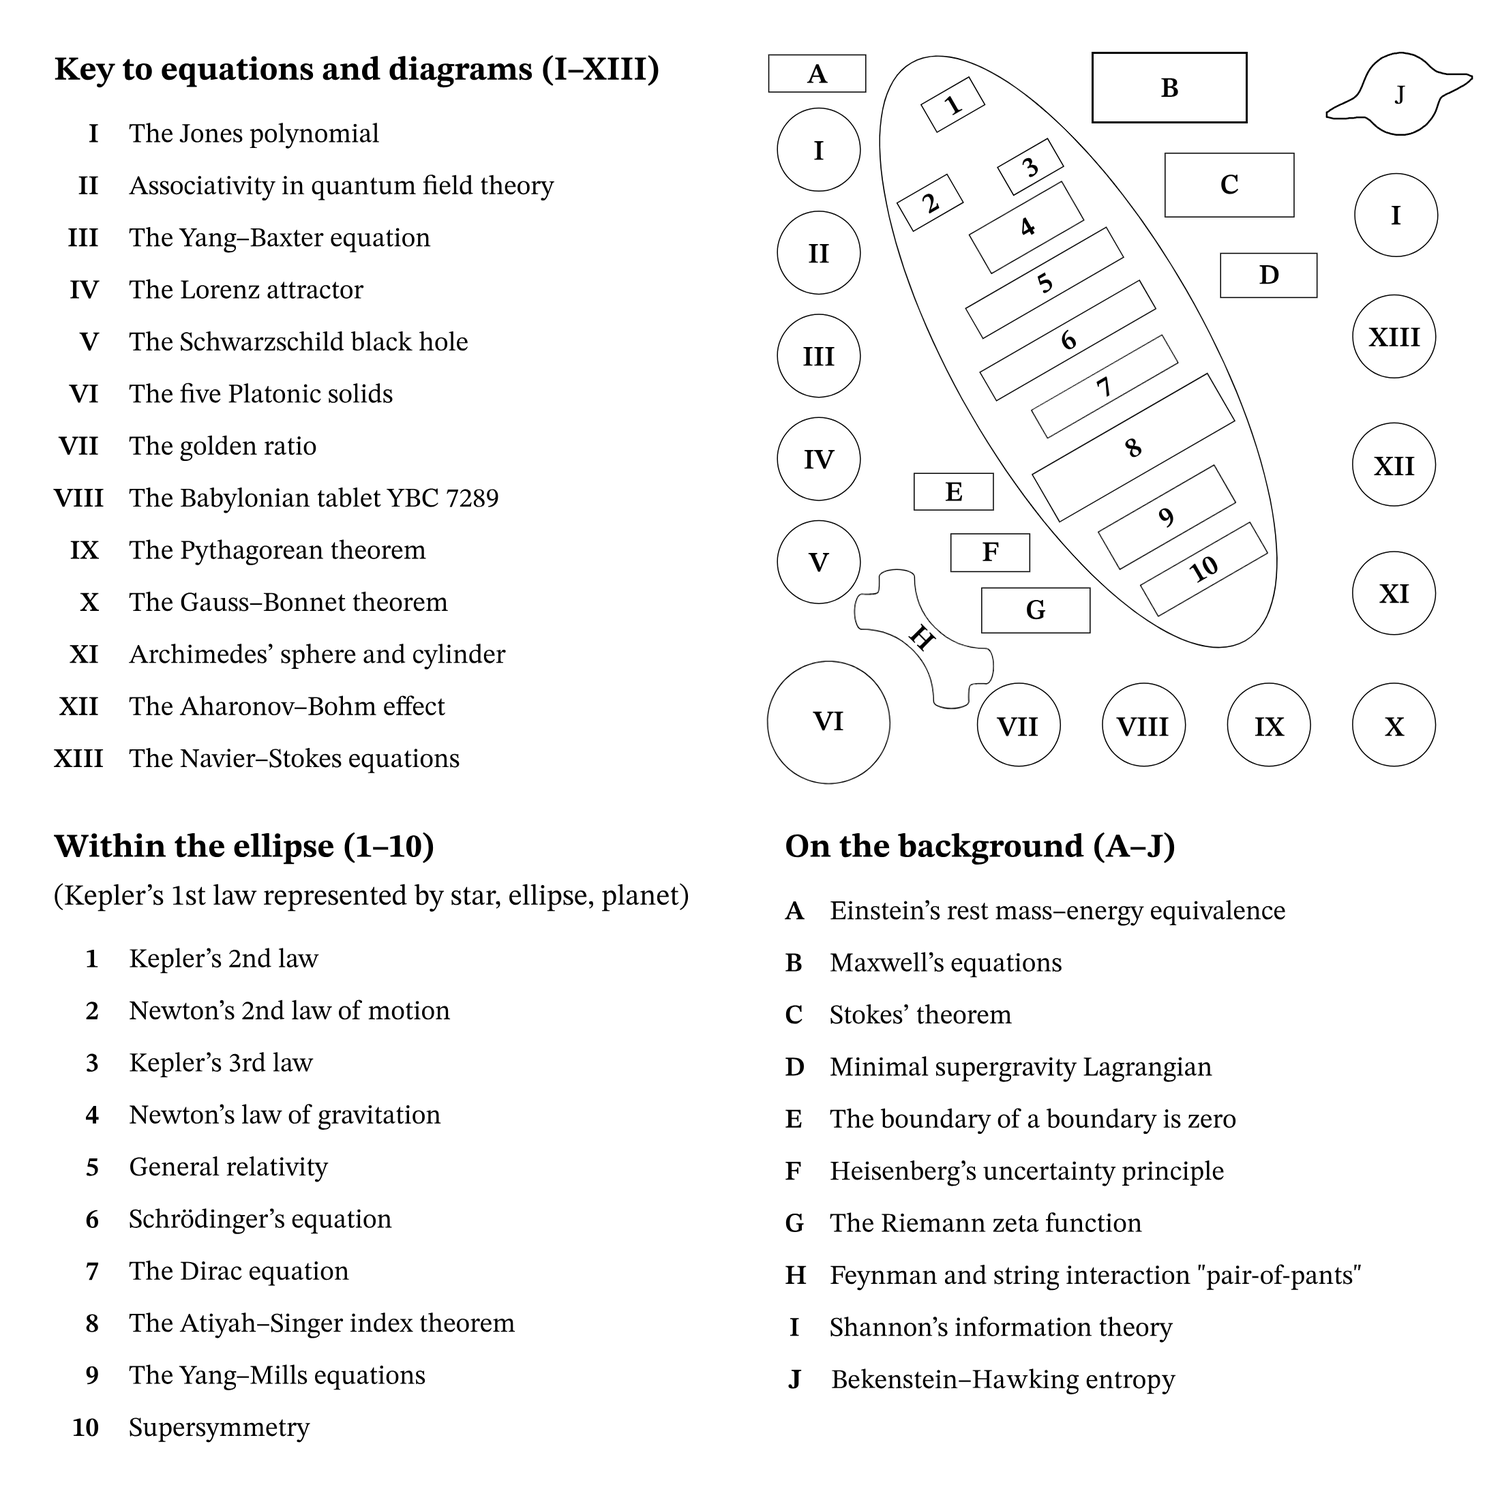
\includegraphics[width=0.66\linewidth]{legend-plaque.png}
  \vspace{-4pt}
  \caption{The $10\times10$ legend plaque, August 2026 revision. The
    locator mirrors the July 31 wall: the Bekenstein--Hawking entry (J)
    appears as its black-hole silhouette at the top right, with Shannon
    (I) and Navier--Stokes (XIII) following down the right edge.}
\end{figure}

\newpage
% ============================================================ APPENDIX C
\head{Appendix C\quad Element-by-element changes}
The following tables list every named item in the original key, the ten
ellipse items, and every background item. ``Retained'' does not mean
visually identical; in nearly every case the final version was redrawn
or retypeset as consistent black vector art.

\subsection*{C.1\quad Peripheral diagrams and medallions (I--XIII)}
\renewcommand{\arraystretch}{1.22}
\begin{longtable}{@{}L{2.55cm} L{4.6cm} L{5.5cm} L{2.9cm}@{}}
\toprule
\textbf{Item} & \textbf{Original reference} & \textbf{Final version} & \textbf{Change type}\\
\midrule
\endhead
I~Jones polynomial & Trefoil knot ringed by $V_K(t)$ and Witten's
  Chern--Simons path integral. & Notation rewritten to Wilson-loop form
  $\langle W(K)\rangle_k$ with $q = e^{2\pi i/(k+2)}$ stated separately;
  redrawn as vector line art (\S3.1). & Notation change, redraw.\\
II~Associativity in QFT & Tree-level associativity diagram. & Retained;
  redrawn. & Redraw, typography.\\
III~Yang--Baxter equation & Braiding equality diagram with $R$-matrix
  expression. & Retained; redrawn. & Redraw, typography.\\
IV~Lorenz attractor & Butterfly image credited to Scott Sutherland. &
  Redrawn as vector attractor; the three equations are symbol-for-symbol
  unchanged (letterforms and spacing only); credit removed. & Photo to
  vector.\\
V~Schwarzschild black hole & Embedding-diagram medallion. & Retained;
  redrawn with clean vector curves. & Redraw, spelling check.\\
VI~Five Platonic solids & Five separate solid diagrams. & Retained;
  redrawn with consistent outlines. & Redraw.\\
VII~Golden ratio & Golden rectangle/spiral with limit and continued
  fraction. & Retained; redrawn. & Redraw, typography.\\
VIII~Babylonian tablet & Tablet photograph credited to Bill Casselman.
  & Simplified line-art tablet medallion; credit removed. & Photo to
  vector.\\
IX~Pythagorean theorem & Wordless-proof diagrams. & Retained; redrawn.
  & Redraw, typography.\\
X~Gauss--Bonnet theorem & Torus medallion and formula. & Retained;
  cleaner torus and formula placement. & Redraw.\\
XI~Archimedes & ``Calculation of the volume and area of the sphere'';
  formula shown generically. & Label shortened; formula clarified as
  the sphere--cylinder relationship, $V_s=\tfrac{2}{3}V_c$,
  $A_s=\tfrac{2}{3}A_{c,\mathrm{tot}}$. & Label, notation.\\
XII~Aharonov--Bohm effect & Magnetic flux-tube and path diagram. &
  Retained; formula and paths cleaned. & Redraw, typography.\\
XIII~Navier--Stokes & Flow image credited to J.D. Kim / AMS / Stony
  Brook. & Vectorized line-art vortex; credit removed; repositioned to
  the right edge, below Shannon's block (July 31 layout). & Image to
  vector.\\
\bottomrule
\end{longtable}

\subsection*{C.2\quad Ellipse items (Kepler + 1--10)}
\begin{longtable}{@{}L{2.55cm} L{4.6cm} L{5.5cm} L{2.9cm}@{}}
\toprule
\textbf{Item} & \textbf{Original} & \textbf{Final} & \textbf{Change type}\\
\midrule
\endhead
Kepler's 1st law & Star, ellipse, planet represented compositionally. &
  Retained; ellipse and sun lines cleaned in the square layout. &
  Redraw, layout.\\
1~Kepler's 2nd law & $\mathrm{d}\theta/\mathrm{d}t \propto 1/r^2$. &
  Retained; retypeset and repositioned. & Typographic cleanup.\\
2~Newton's 2nd law & $F = ma$. & Retained; legend ``Second''
  $\rightarrow$ ``2nd''. & Legend style.\\
3~Kepler's 3rd law & $T^2 \propto a^3$. & Retained; retypeset. &
  Typographic cleanup.\\
4~Newton's gravitation & $F = G m_1 m_2 / r^2$. & Retained; retypeset.
  & Typographic cleanup.\\
5~General relativity & Einstein field equation. & Retained; retypeset
  with cleaner spacing. & Typographic cleanup.\\
6~Schr\"odinger equation & Nonrelativistic Schr\"odinger equation. &
  Retained; clearer $\hbar$, Laplacian, and potential notation. &
  Typographic cleanup.\\
7~Dirac equation & $(i\slashed{D} - m)\psi = 0$ (compact slashed
  form). & $(i\gamma^\mu \partial_\mu - m)\psi = 0$ (explicit form,
  \S3.3). & Notation change.\\
8~Atiyah--Singer & Index formula. & Retained; retypeset. & Typographic
  cleanup.\\
9~Yang--Mills & $F = \mathrm{d}A + A\wedge A$;\ $D_A^{*} F_A = 0$
  (stone carves the first $F$ bare; the catalogue typesets $F_A$). &
  $F_A = \mathrm{d}A + A\wedge A$;\ $\mathrm{d}_A^{*} F_A = 0$
  (\S3.4). & Subscripts, operator case.\\
10~Supersymmetry & $\{Q, Q\} = P$ schematic. &
  $\{Q_\alpha, \bar{Q}_{\dot{\beta}}\} =
  2(\sigma^\mu)_{\alpha\dot{\beta}} P_\mu$ (\S3.5). & Formula made
  explicit.\\
\bottomrule
\end{longtable}

\subsection*{C.3\quad Background items (A--J)}
\begin{longtable}{@{}L{2.55cm} L{4.6cm} L{5.5cm} L{2.9cm}@{}}
\toprule
\textbf{Item} & \textbf{Original} & \textbf{Final} & \textbf{Change type}\\
\midrule
\endhead
A~Mass--energy & Background label ``E=mc\textsuperscript{2}''. & Legend
  reads ``Einstein's rest mass--energy equivalence''; artwork uses
  $E_0 = mc^2$. & Name, rest-energy notation.\\
B~Maxwell's equations & Four equations: $\nabla\times B =
  \frac{1}{c}\partial E/\partial t$, $\nabla\times E =
  -\frac{1}{c}\partial B/\partial t$, $\nabla\cdot B = 0$,
  $\nabla\cdot E = 0$. & Recast as $\mathrm{d}F = 0$ and
  $\mathrm{d}{\star}F = {\star}J$ in one compact block. & Vector
  calculus $\rightarrow$ differential forms (July 2026).\\
C~Stokes' theorem & Integral formula. & Retained; retypeset. &
  Typographic cleanup.\\
D~Supergravity & Generic ``Supergravity'' label and formula. & Legend
  specifies ``Minimal supergravity Lagrangian''; formula redrawn beside
  the Dynkin diagram. & Label specificity, redraw.\\
E~Boundary of a boundary & $\partial\partial = 0$. & $\partial^2 = 0$
  (\S3.2). & Equivalent, more compact.\\
F~Heisenberg uncertainty & $\Delta x\,\Delta p \ge \hbar/2$. &
  Retained; retypeset. & Typographic cleanup.\\
G~Riemann zeta & Euler product--sum relationship, product on the left:
  $\prod_p \frac{1}{1-1/p^s} = \sum_{n=1}^{\infty} \frac{1}{n^s}$. &
  Sides exchanged --- the artwork reads
  $\sum_{n=1}^{\infty} \frac{1}{n^s} = \prod_p \frac{1}{1-1/p^s}$;
  retypeset. & Order, typography.\\
H~Feynman diagrams & Particle diagram and string-interaction detail. &
  Legend expanded to ``Feynman and string interaction
  pair-of-pants''. & Label expanded.\\
I~Shannon & \emph{No original entry.} & New block:
  $H(p) = -\sum_i p_i \log_2 p_i$ with carved binary strings. & New
  content.\\
J~Bekenstein--Hawking & \emph{No original entry.} & New medallion at
  the top right of the wall: a black hole ringed by its accretion disc,
  with $S = k_B A c^3\!/\,4G\hbar$ inscribed on the event horizon ---
  gravity, quantum mechanics, thermodynamics, and information in one
  line. & New content (July 2026); pictorial black-hole medallion (July
  31, 2026).\\
\bottomrule
\end{longtable}

\end{document}
